
\chapter{Least squares and Singular Values}
\label{sec:leastsquaresSVD}
\index{Least squares}

Consider the linear algebraic equation $L(x)=v$, where $L \colon U\stackrel{\text{linear}}{-\!\!\!-\!\!\!\longrightarrow}W$ and $v\in W$ are known while $x$ is unknown. As we have seen, this system may have 
one solution, no solutions, or infinitely many solutions.  
But if $v$ is not in the range of $L$ there will {\it never} be any solutions for $L(x)=v$.
\vspace{-.1cm}
\begin{center}
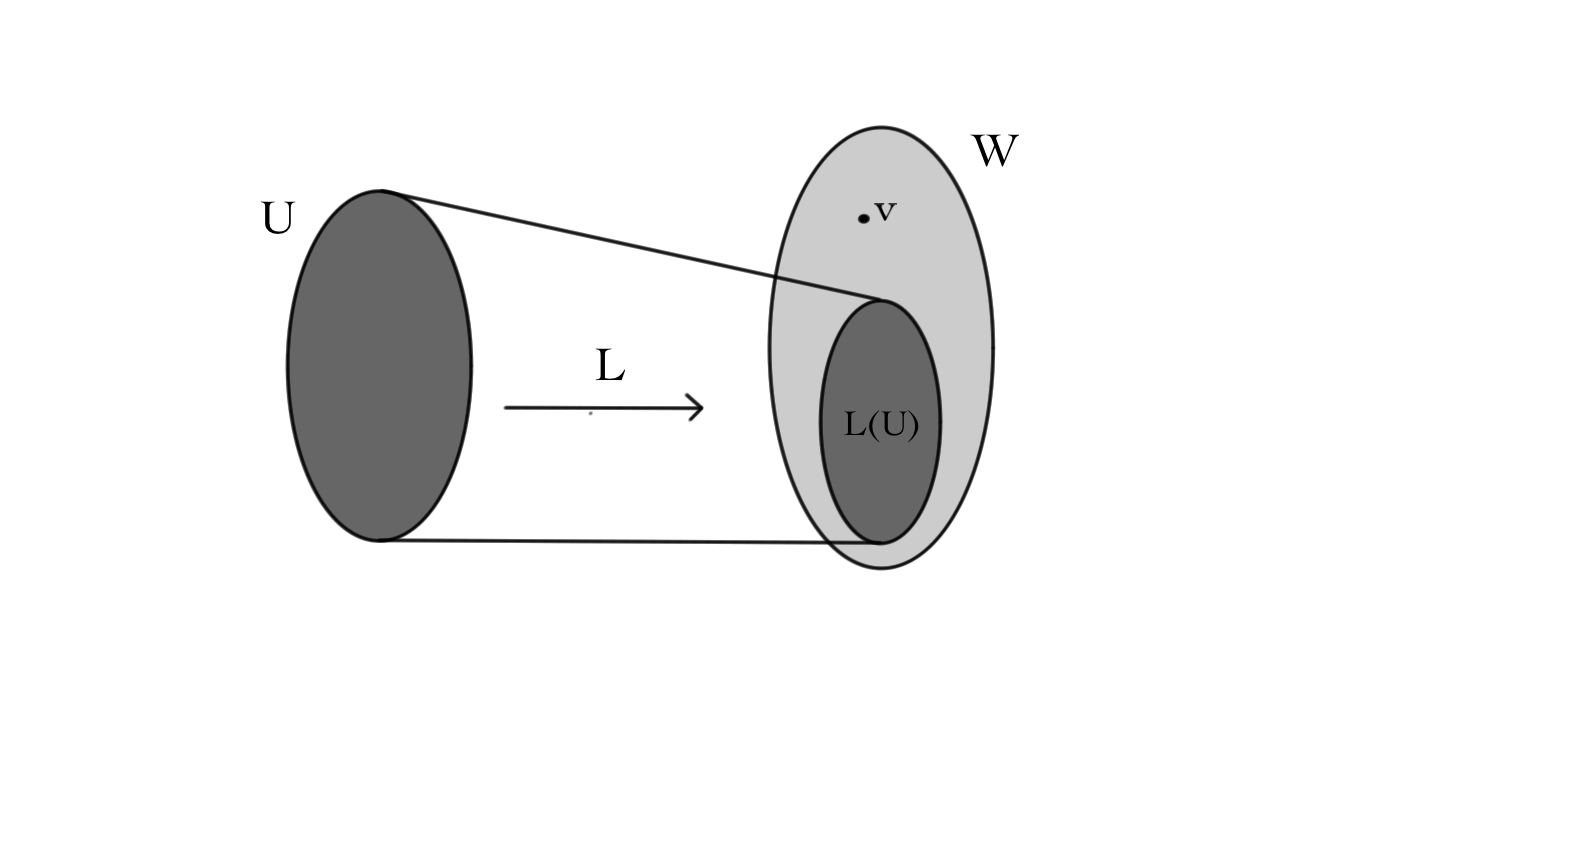
\includegraphics[scale=.24]{notinimage.jpg}
\end{center} 
\vspace{-1.8cm}
However, for many applications we do not need an exact solution of the system; instead, we may only need the best approximation possible.  

\begin{quote}
``My work always tried to unite the Truth with the Beautiful, but when I had to choose one or the other, I usually chose the Beautiful.'' 

\vspace{-2mm}
\hspace{7cm}-- Hermann Weyl.
\end{quote}

If the vector space $W$ has a notion of lengths of vectors, we can try to find $x$ that minimizes $||L(x)-v||$.
\begin{center}
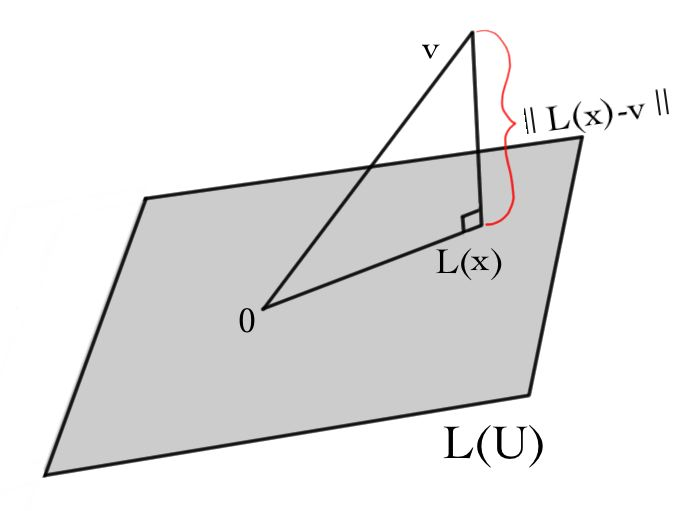
\includegraphics[scale=.24]{minimize.jpg}
\end{center} 
This method has many applications, such as when trying to fit a (perhaps linear) function to a ``noisy'' set of observations.  For example, suppose we measured the position of a bicycle on a racetrack once every five seconds.  Our observations won't be exact, but so long as the observations are right on average, we can figure out a best-possible linear function of position of the bicycle in terms of time.

Suppose $M$ is the matrix for the linear function $L:U \to W$ in some bases for $U$ and $W$. The vectors~$v$ and~$x$ are represented by column vectors $V$ and $X$ in these bases.  Then we need to approximate
\[
MX-V\approx 0\, .
\]

Note that if $\dim U=n$ and $\dim W=m$ then $M$ can be represented by an $m\times n$ matrix and $x$ and $v$ as vectors in $\Re^n$ and $\Re^m$, respectively. Thus, we can write $W=L(U)\oplus L(U)^\perp$.  Then we can uniquely write $v=v^\parallel + v^\perp$, with $v^\parallel \in L(U)$ and $v^\perp \in L(U)^\perp$.  



Thus we should solve $L(u)=v^\parallel$.  In components, $v^\perp$ is just $V-MX$, and is the part we will eventually wish to minimize.  

In terms of $M$, recall that $L(V)$ is spanned by the columns of $M$.  (In the standard basis, the columns of $M$ are $Me_1$, 
$\ldots$, $Me_n$.)  Then $v^\perp$ must be perpendicular to the columns of $M$.  \textit{i.e.}, $M^T(V-MX)=0$, or
\[
M^TMX = M^TV.
\]
Solutions of $M^TMX = M^TV$ for $X$ are called \emph{least squares}\index{Least squares!solutions} solutions to $MX=V$.  
Notice that any solution $X$ to $MX=V$ is a least squares solution.  However, the converse is often false.  In fact, the equation $MX=V$ may have no solutions at all, but still have least squares solutions to $M^TMX = M^TV$.

Observe that since $M$ is an $m\times n$ matrix, then $M^T$ is an $n\times m$ matrix.  Then $M^TM$ is an $n\times n$ matrix, and is symmetric, since $(M^TM)^T=M^TM$.  Then, for any vector $X$, we can evaluate $X^TM^TMX$ to obtain a number.  This is a very nice number, though!  It is just the length $|MX|^2 = (MX)^T(MX)=X^TM^TMX$.

%\href{\webworkurl ReadingHomework25/1/}{Reading homework: problem 25.1}
\Reading{LeastSquares}{1}

Now suppose that $\ker L=\{0\}$, so that the only solution to $MX=0$ is $X=0$. (This need not mean that $M$ is invertible because $M$ is an $n\times m $ matrix, so not necessarily square.) 
However the square matrix $M^TM$ {\it is} invertible. To see this, suppose there was a vector $X$ such that 
$M^T M X=0$. Then it would follow that $X^T M^T M X = |M X|^2=0$. In other words the vector $MX$ would have zero length, so could only be the zero vector. But we are assuming that $\ker L=\{0\}$ so $MX=0$ implies $X=0$. Thus the kernel of $M^TM$ is $\{0\}$ so this matrix is invertible.
So, in this case, the least squares solution (the $X$ that solves $M^TMX=MV$) is unique, and is equal to 
\[
X = (M^TM)^{-1}M^TV.
\]
In a nutshell, this is the least squares method:

\begin{itemize}
\item Compute $M^TM$ and $M^TV$.
\item Solve $(M^TM)X=M^TV$ by Gaussian elimination.
\end{itemize}


\begin{example}
Captain Conundrum\index{Captain Conundrum} falls off of the leaning tower of Pisa and makes three (rather shaky) measurements of his velocity at three different times.

\begin{center}
\begin{tabular}{c|c}
$t$ s & $v $ m/s \\ \hline
$1$ & $11$ \\
$2$ & $19$ \\
$3$ & $31$
\end{tabular}
\end{center}

Having taken some calculus\footnote{In fact, he is a \emph{Calculus Superhero}\index{Calculus Superhero}.}, he believes that his data are best approximated by a straight line
\[
v = at+b.
\]
Then he should find $a$ and $b$ to best fit the data.
\begin{eqnarray*}
11 &=& a\cdot 1 + b \\
19 &=& a\cdot 2 + b \\
31 &=& a\cdot 3 + b.
\end{eqnarray*}
As a system of linear equations, this becomes:

\[
\begin{pmatrix}
1 & 1 \\
2 & 1 \\
3 & 1 \\
\end{pmatrix}
\colvec{a\\b} \stackrel{?}{=}
\colvec{11\\19\\31}.
\]
There is likely no actual straight line solution, so instead solve $M^TMX=M^TV$.

\[
\begin{pmatrix}
1 & 2 & 3 \\
1 & 1 & 1 \\
\end{pmatrix}
\begin{pmatrix}
1 & 1 \\
2 & 1 \\
3 & 1 \\
\end{pmatrix} \colvec{a\\b}
= 
\begin{pmatrix}
1 & 2 & 3 \\
1 & 1 & 1 \\
\end{pmatrix}
\colvec{11\\19\\31}.
\]
This simplifies to 

\[
\begin{amatrix}{2}
14 & 6 & 142 \\
6 & 3 & 61
\end{amatrix}
\sim
\begin{amatrix}{2}
1 & 0 & 10 \\
0 & 1 & \frac{1}{3}
\end{amatrix}.
\]
Thus, the least-squares fit is the line

\[
v = 10\ t + \frac{1}{3}\, .
\]
Notice that this equation implies that Captain Conundrum accelerates towards Italian soil at 10 m/s$^2$ (which is an excellent
approximation to reality) and that he started at a downward velocity of $\frac13$ m/s (perhaps somebody gave him a shove...)!

\end{example}

\section{Projection Matrices}
We have seen that even if $MX=V$ has no solutions $M^TMX=M^T V$ does have solutions. One way to think about this is, since the codomain of $M$ is the direct sum 
$$ \text{codom M}=\text{ran} M \oplus \ker M^T$$ 
there is a unique way to write  $V=V_r+V_k$ with $V_k\in \ker M^T$ and $V_r\in \text{ran }\, M$, and it is clear that $Mx=V$ only has a solution of 
$V\in \text{ran}\, M \Leftrightarrow V_k=0$. If not, then the closest thing to a solution of $MX=V$ is a solution to $MX=V_r$. We learned to find solutions to this in the previous subsection of this book. 

But here is another question, how can we determine what $V_r$ is given $M$ and $V$? The answer is simple; suppose $X$ is a solution to $MX=V_r$. Then
$$  MX=V_r 
\implies M^TMx=M^T V_r 
\implies M^TMx=M^T (V_r + 0) $$ 
$$
\implies M^TMx=M^T (V_r+V_k)
\implies M^TMx=M^T V 
\implies X=(M^TM)^{-1} M^T V 
$$
if indeed $M^TM$ is invertible. Since, by assumption, $X$ is a solution \\
\begin{center}
\shabox{ $M(M^TM)^{-1} M^T\, V =V_r. $}
\end{center}
That is, the matrix which projects $V$ onto its $\text{ran} \, M$ part is $M(M^TM)^{-1} M^T$. 

\begin{example} To project $\colvec{1\\1\\1}$ onto $\spa \left\{    \colvec{ 1\\1\\0}, \colvec{1\\-1\\0 }  \right\} = \text{ran} 
\begin{pmatrix}
 1& 1  \\
1 & -1  \\
0 & 0 
\end{pmatrix}
 $ 
  multiply by the matrix 
 $$
\begin{pmatrix}
 1& 1  \\
1 & -1  \\
0 & 0 
\end{pmatrix}
\left [ 
 \begin{pmatrix}
 1& 1 &0 \\
1 & -1 &0 
\end{pmatrix}
\begin{pmatrix}
 1& 1  \\
1 & -1  \\
0 & 0 
\end{pmatrix}
 \right]^{-1}
 \begin{pmatrix}
 1& 1 &0 \\
1 & -1 &0 
\end{pmatrix}
 $$
 $$
=\begin{pmatrix}
 1& 1  \\
1 & -1  \\
0 & 0 
\end{pmatrix}
 \begin{pmatrix}
 2& 0  \\
0 & 2  
\end{pmatrix}^{-1}
 \begin{pmatrix}
 1& 1 &0 \\
1 & -1 &0 
\end{pmatrix} 
$$
$$
=\frac12 \begin{pmatrix}
 1& 1  \\
1 & -1  \\
0 & 0 
\end{pmatrix}
 \begin{pmatrix}
 1& 1 &0 \\
1 & -1 &0 
\end{pmatrix} 
=
\frac12 \begin{pmatrix}
 2 & 0 &0 \\
0 & 2  &0\\
0 & 0 &0
\end{pmatrix}. 
$$

This gives 
$$\frac12 \begin{pmatrix}
 2 & 0 &0 \\
0 & 2  &0\\
0 & 0 &0
\end{pmatrix}
\colvec{1\\1\\1 } = \colvec{1\\1\\0} .$$
\end{example}



\section{Singular Value Decomposition}

Suppose 
$$
L:V\tolinear W\, .
$$
It is unlikely that $\dim V=:n=m:=\dim W$ so a $m\times n$ matrix $M$ of $L$ in bases for $V$ and $W$ will not be square.
Therefore there is no eigenvalue problem  we can use to uncover a preferred basis. However, if the vector spaces $V$ and 
$W$ both have inner products, there does exist an analog of the eigenvalue problem, namely the singular values of $L$.

Before giving the details of the powerful technique known as the singular value decomposition, we note that it is an 
excellent example of what Eugene Wigner called the ``Unreasonable Effectiveness of Mathematics'':
\begin{quote}{\scriptsize
There is a story about two friends who were classmates in high school, talking about their jobs. One of them became a statistician
and was working on population trends. He showed a reprint to his former classmate.
The reprint started, as usual with the Gaussian distribution and the statistician explained
to his former classmate the meaning of the symbols for the actual population and so on. His classmate
was a bit incredulous and was not quite sure whether the statistician was pulling his leg. ``How can you 
know that?'' was his query. ``And what is this symbol here?'' ``Oh,'' said the statistician, this is ``$\pi$.''
``And what is that?'' ``The ratio of the circumference of the circle to its diameter.'' ``Well, now
you are pushing your joke too far,'' said the classmate, ``surely the population has nothing to do with the 
circumference of the circle.''


Eugene Wigner, Commun. Pure and Appl. Math. {\bf XIII}, 1 (1960).
}
\end{quote}
Whenever we mathematically model a system, any ``canonical quantities'' 
(those that  %on which we can all agree and 
do not
depend on any choices we make for calculating them) will correspond to important features of the system. For examples, the eigenvalues
of the eigenvector equation you found in review question~\ref{stringval}, chapter~\ref{eigenvalseigenvects} encode the notes and harmonics that a guitar string can play! 

Singular values appear in many linear algebra applications, especially those involving very large data sets such as statistics and signal processing. 

Let us focus on the $m\times n$ matrix $M$ of a linear transformation $L:V\to W$ written in orthonormal bases for the input and outputs of $L$ (notice, the existence of these othonormal bases is predicated on having inner products for $V$ and $W$).
Even though the matrix $M$ is not square, both the matrices $M M^T$ and $M^T M$ are square and symmetric! 
In terms of linear transformations $M^T$ is the matrix of a linear transformation 
$$
L^*:W\tolinear V\, .
$$
Thus $LL^*:W\to W$ and $L^*L:V\to V$ and both have eigenvalue problems.
Moreover,  as is shown  in Chapter~\ref{symmetricmatrices},  both $L^*L$ and $LL^*$ have orthonormal bases of eigenvectors, and
 both $MM^T$ and $M^TM$ can be diagonalized. 
 
Next, let us make a simplifying assumption, namely $\ker L=\{0\}$. This is not necessary, but will make some of our computations simpler.
Now suppose we have found an orthonormal basis $(u_1,\ldots , u_n)$ for $V$ composed of eigenvectors for $L^*L$. That is 
$$
L^*L u_i= \lambda_i u_i\, .
$$
Then multiplying by $L$ gives 
$$
L L^* L u_i = \lambda_i L u_i\, .
$$
{\it I.e.}, $L u_i$ is an eigenvector of $L L^*$.
The vectors $(Lu_1,\ldots, Lu_n)$ are linearly independent, because $\ker L=\{0\}$ (this is where we use our simplifying assumption, but you can 
try and extend our analysis to the case where it no longer holds). 

Lets compute the angles between and lengths of these vectors. 
For that we express the vectors $u_i$ in the bases used to compute the matrix $M$ of $L$. Denoting these column vectors by $U_i$ we then compute
$$
(MU_i)\cdot (MU_j)=U_i^T M^T M U_j = \lambda_j \, U_i^T U_j=\lambda_j \, U_i\cdot U_j = \lambda_j \delta_{ij}\, .
$$
We see that  vectors $(Lu_1,\ldots, Lu_n)$ are orthogonal but not orthonormal. Moreover, the length of $Lu_i$ is $\sqrt{\lambda_i}$.
Normalizing gives the orthonormal and linearly independent ordered set
$$
\left(\frac{Lu_1}{\sqrt{\lambda_1}},\ldots,\frac{Lu_n}{\sqrt{\lambda_n}}\right).
$$

In general, this cannot be a basis for $W$ 
since $\ker L=\{0\},~\dim L(V)=\dim V,$
and in turn $\dim V\leq \dim W$, so $n\leq m$. 

However,  it is a subset of the eigenvectors of $LL^*$ so there is an orthonormal basis of eigenvectors of $LL^*$ of the form 
$$
O'=\left(\frac{Lu_1}{\sqrt{\lambda_1}},\ldots,\frac{Lu_n}{\sqrt{\lambda_n}},v_{n+1},\ldots,v_{m}\right)=:(v_1,\ldots,v_m)\, .
$$
Now lets compute the matrix of $L$ with respect to the orthonormal basis $O=(u_1,\ldots,u_n)$ for $V$ and the orthonormal basis~$O'=(v_1,\ldots,v_m)$ for~$W$. As usual, our starting point is the computation of $L$ acting on the input basis vectors;
\begin{eqnarray*}
LO=\big(Lu_1,\ldots, Lu_n\big)&=&
\big(\sqrt{\lambda_1}\,  v_1,\ldots,\sqrt{\lambda_n}\,  v_n\big)\\[2mm]&=&\big(v_1,\ldots,v_m\big)
%\begin{pmatrix}
%\sqrt{\lambda_1}&\mc0&\cdots&\mc0&0&\cdots&0\\[1mm]
%\mc0&\sqrt{\lambda_2}&\cdots&\mc0&0&\cdots&0\\
%\mc{\vdots}&\mc\vdots&\ddots&\mc\vdots&\mc\vdots&&\mc\vdots\\[1mm]
%\mc0&\mc0&\cdots&\sqrt{\lambda_n}&0&\cdots&0\\
%\end{pmatrix}
\begin{pmatrix}
\sqrt{\lambda_1}&\mc0&\cdots&\mc0\\[1mm]
\mc0&\sqrt{\lambda_2}&\cdots&\mc0\\
\mc{\vdots}&\mc\vdots&\ddots&\mc\vdots\\[1mm]
\mc0&\mc0&\cdots&\sqrt{\lambda_n}\\[1mm]
\mc 0 & \mc 0& \cdots &\mc 0\\
\mc{\vdots}&\mc\vdots&&\mc\vdots\\
\mc 0 & \mc 0& \cdots &\mc 0
\end{pmatrix}\, .
\end{eqnarray*}
The result is very close to diagonalization; the numbers $\sqrt{\lambda_i}$ along the leading diagonal are called the singular values of $L$.

\begin{example} Let the matrix of a linear transformation be
$$
M=\begin{pmatrix}
\frac12&\frac12\\[1mm]-1&1\\[1mm]-\frac12&-\frac12
\end{pmatrix}\, .
$$
Clearly $\ker M=\{0\}$ while
$$
M^TM=\begin{pmatrix}\frac32&-\frac12\\[2mm]-\frac12&\frac32\end{pmatrix}
$$
which has eigenvalues and eigenvectors
$$
 \lambda=1\, ,\,  u_1:=\colvec{\frac{1}{\sqrt2}\\[2mm]\frac{1}{\sqrt2}}; \qquad
\lambda=2\, ,\,  u_2:=\colvec{\frac{1}{\sqrt2}\\[2mm]-\frac{1}{\sqrt2}}\,\, .
$$
so our orthonormal input basis is $$O=\left(\colvec{\frac{1}{\sqrt2}\\[2mm]\frac{1}{\sqrt2}},\colvec{\frac{1}{\sqrt2}\\[2mm]-\frac{1}{\sqrt2}}\right)\, .
$$
These are called the {\it right singular vectors}\index{Right singular vector} of $M$.
The vectors 
$$
M u_1= \colvec{\frac1{\sqrt{2}}\\[1mm]\mc{\ \ 0}\\-\frac1{\sqrt{2}}}\mbox{ and }
M u_2=\ccolvec{0\\[1mm]-\sqrt{2}\\[1mm]0}
$$
are eigenvectors of 
$$M M^T=\begin{pmatrix}\frac12&\ 0&\!-\frac12\\0&2&0\\-\frac12&0&\frac12\end{pmatrix}$$ 
with eigenvalues $1$ and $2$, respectively. The third eigenvector (with eigenvalue~$0$) of $MM^T$ is 
$$v_3=\colvec{\frac1{\sqrt{2}}\\[1mm]\mc{\ \ 0}\\ \frac1{\sqrt{2}}}\, .$$
The eigenvectors $Mu_1$ and $Mu_2$ are necessarily orthogonal, dividing them by their lengths we obtain the {\it left singular vectors}\index{Left singular vectors} and in turn  our orthonormal output basis
$$
O'=\left(\colvec{\frac1{\sqrt{2}}\\[1mm]\mc{\ \ 0}\\-\frac1{\sqrt{2}}},\ccolvec{0\\[1mm]-1\\[1mm]0},\colvec{\frac1{\sqrt{2}}\\[1mm]\mc{\ \ 0}\\\frac1{\sqrt{2}}}\right)\, .
$$
The new matrix~$M'$ of the linear transformation given by $M$ with respect to the bases $O$ and $O'$ is
$$
M'=\begin{pmatrix}
1&0\\0&\sqrt{2}\\0&0
\end{pmatrix}\, ,
$$
so the singular values are $1,\sqrt{2}$. 

Finally note that arranging the column vectors of $O$ and $O'$ into change of basis matrices
$$
P=\begin{pmatrix}
\frac1{\sqrt{2}}&\frac1{\sqrt{2}}\\[2mm]
\frac1{\sqrt{2}}&-\frac1{\sqrt{2}}
\end{pmatrix}\, ,\qquad
Q=
\begin{pmatrix}
\frac1{\sqrt{2}}&0&\frac1{\sqrt{2}}\\[2mm]
\mc {\ \ 0}&-1&\mc 0\\[2mm]
\!-\frac1{\sqrt{2}}&0&\frac1{\sqrt{2}}
\end{pmatrix}\, ,
$$
we have, as usual,
$$
M'=Q^{-1}MP\, .
$$
\end{example}

Singular vectors and values have a very nice geometric interpretation; they provide an orthonormal bases for the domain and range of $L$
and give the factors by which $L$ stretches the orthonormal input basis vectors. This is depicted below for the example we just computed.
\begin{center}
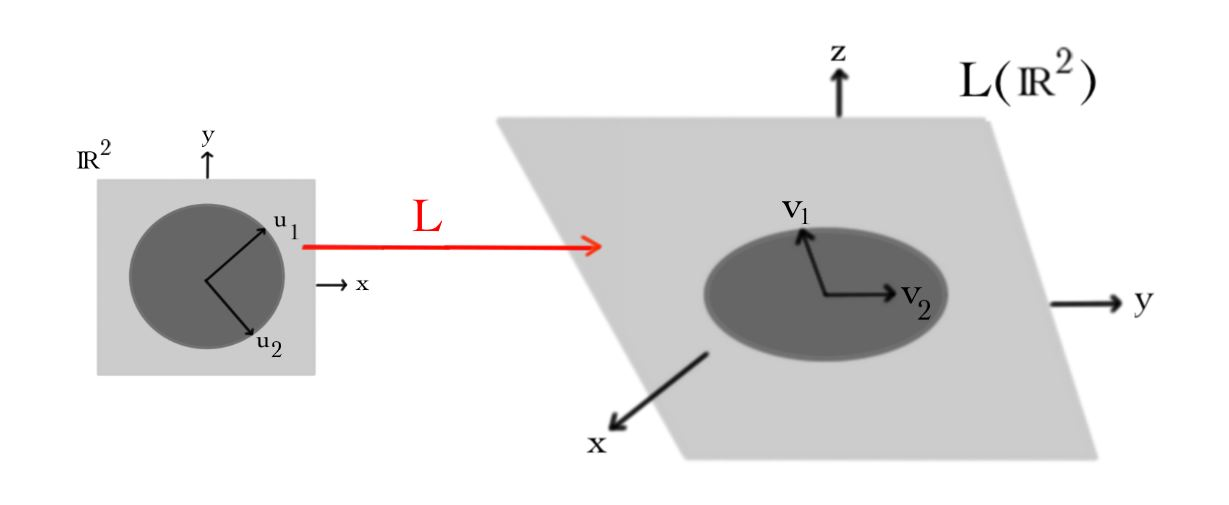
\includegraphics[scale=.27]{singval.jpg}
\end{center} 



%{\it Congratulations, you have reached the end of these notes! You can test your skills
%on the \hyperref[sample3]{sample final exam}.}
\begin{center}
\shabox{
{\bf \hyperref[sample3]{\begin{tabular}{c}Congratulations, you have reached the end of the book! \\[2mm]
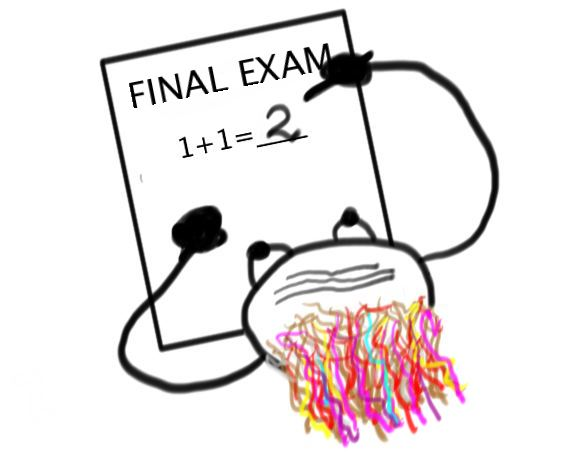
\includegraphics[scale=.15]{final.jpg}\\
Now test your skills on the \hyperref[sample3]{sample final exam}.
%You are now ready to 
%apply for membership in\\
% be a minion of Captain Conundrum's nemesis, 
%The League of Ninjas of Numbers. 
%Now test your skills
%on the sample final exam. 
\end{tabular}
}}}
\end{center}













%\section*{References}
%Hefferon, Chapter Three, Section VI.2: Gram-Schmidt Orthogonalization \\
%Beezer, Part A, Section CF, Subsection DF \\
%Wikipedia:
%\begin{itemize}
%\item \href{http://en.wikipedia.org/wiki/Linear_least_squares}{Linear Least Squares}
%\item \href{http://en.wikipedia.org/wiki/Least_squares}{Least Squares}
%\end{itemize}

\section{Review Problems}

{\bf Webwork:} 
\begin{tabular}{|c|c|}
\hline
Reading Problem & 
 \hwrref{LeastSquares}{1}, 
\\
   \hline
\end{tabular}





\begin{enumerate}

\item While performing  Gaussian elimination on these augmented matrices write the full system of equations describing the new rows in terms of the old rows above each equivalence symbol as in  \hyperlink{Keeping track of EROs with equations between rows}{Example}~\ref{Rsystem}. 
$$
\begin{amatrix}{2} 
2 & 2 & 10 \\
1 & 2 & 8 \\
\end{amatrix}
,~
\begin{amatrix}{3} 
1 & 1 & 0 & 5 \\
1 & 1 & \!\!-1& 11 \\
-1 & 1 & 1 & -5 \\ 
\end{amatrix}
$$

%%%%%%%%%%%%%%%%%%%

\item Solve the vector equation by applying ERO matrices to each side of the equation to perform elimination. Show each matrix explicitly as in \hyperlink{Undoing}{Example~\ref{slowly}}.

\begin{eqnarray*}
\begin{pmatrix}
3	&6 	&2 \\ %-3
5 	&9 	&4 \\ %1
2	&4	&2 \\ %0
\end{pmatrix} 
\begin{pmatrix}
 x \\ 
y \\
z 
\end{pmatrix} 
=
\begin{pmatrix}
-3 \\ 
1  \\
0  \\
\end{pmatrix} 
\end{eqnarray*}

%%%%%%%%%%%%%%%%%%%

\item Solve this vector equation by finding the inverse of the matrix through $(M|I)\sim (I|M^{-1})$ and then applying $M^{-1}$ to both sides of the equation. 
\begin{eqnarray*}
\begin{pmatrix}
2	&1 	&1 \\ %9
1 	&1 	&1 \\ %6
1	&1	&2 \\ %7
\end{pmatrix} 
\begin{pmatrix}
 x \\ 
y \\
z 
\end{pmatrix} 
=
\begin{pmatrix}
9 \\ 
6  \\
7  \\
\end{pmatrix} 
\end{eqnarray*}


%%%%%%%%%%%%%%%%%%%

\item Follow the method of  \hyperlink{elldeeeww}{Examples~\ref{factorize} and~\ref{factorizes}} to find the $LU$ and $LDU$ factorization of 
\begin{eqnarray*}
\begin{pmatrix}
3	&3 	&6 \\ %0 %2
3 	&5 	&2 \\ %1 %1
6	&2	&5 \\ %0 %1
\end{pmatrix} .
\end{eqnarray*}



%%%%%%%%%%%%%%%%%%%%

\item 
Multiple matrix equations with the same matrix can be solved simultaneously. 
\begin{enumerate}
\item Solve both systems by performing elimination on just one augmented matrix.
\begin{eqnarray*}
\begin{pmatrix}
2	&-1 	&-1 \\ %0 %2
-1 	&1 	&1 \\ %1 %1
1	&-1	&0 \\ %0 %1
\end{pmatrix} 
\begin{pmatrix}
 x \\ 
y \\
z 
\end{pmatrix} 
=
\begin{pmatrix}
0\\ 
1  \\
0  \\
\end{pmatrix} 
,~
\begin{pmatrix}
2	&-1 	&-1 \\ %0 %2
-1 	&1 	&1 \\ %1 %1
1	&-1	&0 \\ %0 %1
\end{pmatrix} 
\begin{pmatrix}
 a \\ 
b \\
c 
\end{pmatrix} 
=
\begin{pmatrix}
2\\ 
1  \\
1  \\
\end{pmatrix} 
\end{eqnarray*}
\item Give an interpretation of the columns of $M^{-1}$ in $(M|I)\sim (I|M^{-1})$ in terms of solutions to certain systems of linear equations.
\end{enumerate}

%%%%%%%%%%%%%%%%%%%%%%%%

\item How can you convince your fellow students to never make this mistake?
\begin{eqnarray*}
\begin{amatrix}{3} 
1 & 0 & 2 & 3 \\ 
0 & 1 & 2& 3 \\
2 & 0 & 1 & 4 \\
\end{amatrix} 
& 
\stackrel{R_1'=R_1+R_2}{
\stackrel{R_2'=R_1-R_2}{ 
\stackrel{\ R_3'= R_1+2R_2}{\sim}}}
&
\begin{amatrix}{3} 
1 & 1 & 4 & 6 \\
1 & \!\!-1 & 0& 0 \\
1 & 2 & 6 & 9 
\end{amatrix}
\end{eqnarray*}

\item Is $LU$ factorization of a matrix unique?  Justify your answer.


\item[$\infty$.] If you randomly create a matrix by picking numbers out of the blue, it will probably be difficult to perform elimination or factorization; fractions and large numbers will probably be involved. To invent simple problems it is better to start with a simple answer:
\begin{enumerate}
\item Start with any augmented matrix in RREF. Perform EROs to make most of the components non-zero. Write the result on a separate piece of paper and give it to your friend. Ask that friend to find RREF of the augmented matrix you gave them. Make sure they get the same augmented matrix you started with.  
\item Create  an upper triangular matrix $U$ and a lower triangular matrix~$L$ with only $1$s on the diagonal. Give the result to a friend to factor into $LU$ form. 
\item Do the same with an $LDU$ factorization. 
\end{enumerate}
\end{enumerate}

\phantomnewpage




\newpage
